En el diseño cinemático del mecanismo resulta de vital importancia un adecuado dimensionamiento de los elementos debido a el impacto que estos tienen en el desempeño del mismo. Esto lleva a buscar una manera de cuantificar y evaluar el desempeño cinemático de los robots por lo cual se propone utilizar alguno índices de desempeños propuestos en la literatura que relacionan las dimensiones y cinemática del mecanismo con el control, precisión, destreza e isotropía por todo el espacio de trabajo. 
Para la evaluación del desempeño cinemático del mecanismo se utiliza el Índice global de desempeño cinemático \citep{zhang2014GlobalI} el cual está basado en la combinación de 4 índices de desempeño cinemático que son:

\textbf{Manipulabilidad}\newline
El índice de manipulabilidad brinda una medida de la capacidad general de posicionamiento y orientación de los actuadores sobre el efector final del mecanismo.
\begin{equation}
    M_{r}= \sqrt[m]{\lambda_1\lambda_2 ..\lambda_m}/l^2 
\end{equation}
$\lambda_i$ son los autovalores del jacobiano\newline
l es la suma de todas las longitudes de los elementos del mecanismo.\newline


\textbf{Velocidad Mínima}\newline
El índice de velocidad minima da un medida de la capacidad de respuesta del efector final en la dirección de menor rendimiento frente a cambios en los actuadores del sistema.
\begin{equation}
    V_{rmin}= \sqrt{min(\lambda_i)}/l
\end{equation}

\textbf{Isotropía de la Velocidad}\newline
El índice de isotropia mide la capacidad de transmisión de movimiento de manera uniforme en todas las direcciones y con un desempeño uniforme para ellas.
\begin{equation}
    \mu_{riso}= \sqrt[m]{\left(\frac{\sigma_1}{\sigma_{avg}}\right)\cdot\left(\frac{\sigma_2}{\sigma_{avg}}\right)...\left(\frac{\sigma_m}{\sigma_{avg}}\right)}
\end{equation}
$\sigma$ son los valores singulares del Jacobiano.\newline


\textbf{Precisión}\newline{}
El índice de precisión está relacionado con los errores de manufactura, errores de ensamblaje y errores en el control de posición. A medida que el índice aumenta la sensibilidad del mecanismo a estos errores es menor, es decir, presenta un mayor rendimiento.
\begin{equation}
    K_j = \frac{1}{||J||\cdot||J^+||}
\end{equation}

La evaluación de cada índice se realiza en todos los puntos del espacio de trabajo de manera discretizada, con los cuales se calcula un índice integral que considera diferentes aspectos de la distribucion del mismo.
\begin{equation}
    \xi_{integr} = (\alpha_1 \cdot\alpha_2\cdot \alpha_3 \cdot\alpha_4)(|\xi_{avg}| |\xi_{vol}| |\xi_{skew}| |\xi_{kurt}| )^T
\end{equation}
Donde:\newline
$\xi_{avg}$ es el valor promedio del índice $\xi$ en el espacio de trabajo. \newline
$\xi_{vol}$ es la volatilidad del índice en el espacio de trabajo. \newline
$\xi_{skew}$ es una medida de la asimetría de la distribución del índice. \newline
$\xi_{kurt}$ es el curtosis de la distribución del índice en el espacio de trabjo. \newline
$\alpha_i$ es el peso relativo de cada parámetro dentro del índice integral. \newline

El índice de desempeño global se calcula considerando los 4 índices calculados previamente
\begin{equation}
    \left(\textbf{GI}_{kine}\right)_{integr} = 
    \frac{\beta_1(M_r)_{integr}}{(M_r)_{norm}} +
    \frac{\beta_2(V_{rmin})_{integr}}{(V_{rmin})_{norm}} +
    \frac{\beta_3(\mu_{riso})_{integr}}{(\mu_{riso})_{norm}} +
    \frac{\beta_4(K_j)_{integr}}{(K_j)_{norm}} 
\end{equation}

Donde:\newline
$\beta_{i}$ es el peso de cada indice dentro del índice Global de Desempeño del mecanismo.\newline

% % % %    GA
En busca del mayor desempeño cinematico posible se desarrolló un algoritmo genetico con el fin de optimizar las dimensiones del mecanismo de forma tal que el Indice Global de Desempeño del robot sea el mayor posible. El algoritmo fue desarrollado en python y se presenta a continuación la rutina principal.

~
\begin{lstlisting}[frame=single,language = python]  % Start your code-block
import numpy as np
import matplotlib.pyplot as plt
import ga
import GlobalIndexKinematical as km

# Variables Range
span = [[500,50,50,-100],
        [1000,250,250,100]]

num_var = 4     #Numero de Variables a Optimizar
num_kromo = 10
pop_size = (num_kromo, 1)

new_pop1 = np.random.uniform(span[0][0], span[1][0], size=pop_size)
new_pop2 = np.random.uniform(span[0][1], span[1][1], size=pop_size)
new_pop3 = np.random.uniform(span[0][2], span[1][2], size=pop_size)
new_pop4 = np.random.uniform(span[0][3], span[1][3], size=pop_size)
new_population = np.concatenate((new_pop1,new_pop2, new_pop3,
                                new_pop4),axis=1)

# Point Cloud - WorkSpace
P = km.WorkspaceDesired(500.0,650.0,50.0)
num_parents = int(num_kromo/2) # Number of Parents
k = 120 # Number of Generations
Global_fitness, Avg_fitness, Mf_chromo=[],[],[]

for i in range(k):
    fitness = ga.fitnessK(new_population,P)
    Global_fitness.append(max(fitness))
    Avg_fitness.append(sum(fitness)/len(fitness))
    parents = ga.select_parents(new_population,fitness,num_parents)
    offspring_cross = ga.crossover(parents,num_kromo)
    mut_prob = 0.6
    offspring_mut = ga.mutation(offspring_cross,span, mut_prob)
    new_population = np.concatenate((parents, offspring_mut))

fitness = ga.fitnessK(new_population,P)
Global_fitness.append(max(fitness))
winner_chromo = new_population[fitness.index(max(fitness))]

win_local_idx = km.AllIndex(winner_chromo,P)
np.savetxt('win_local_idxs.csv', win_local_idx, delimiter = ',')
np.savetxt('Global_idx.csv',Global_fitness, delimiter = ',')
plt.plot(Global_fitness,'b-')
plt.plot(Avg_fitness,'r-')
plt.xlabel('# Generaciones')
plt.show()
\end{lstlisting}

El proceso de optimización con el algoritmo genético inicia con la generación de una poblacion aleatoria de cromosomas, es decir, generar un conjunto de soluciones posibles new\_Population. El siguiente paso es evaluar el desempeño de tal poblacion, para esto se considera el calculo del indice global de desempeño cinematico en los puntos discretizados P del espacio de trabajo. Para cada cromosoma de la población se obtienen los 4 indices descritos previamente, la integracion de estos y el valor del índice global.

\begin{lstlisting}[frame=single,language = python]  % Start your code-block

def fitnessK(population,P):
    fitness_population = []
    for L in population:
        I = km.AllIndex(L,P)
        I = km.IntegratedIndex(I)
        I = km.GlobalIndex(I).tolist()
        fitness_population.append(I[0][0])
    return fitness_population
\end{lstlisting}

A continuación se realiza la selección de los cromosomas elites (aquellos con el desempeño más alto), los cuales sobreviviran y serán base para la generación siguiente.
~
\begin{lstlisting}[frame=single,language = python]  % Start your code-block

def select_parents(pop, fitness, num_parents):
    parents = np.zeros([num_parents,pop.shape[1]])
    for parent_num in range(num_parents):
        max_fit_index = np.where(fitness == np.max(fitness))
        max_fit_index = max_fit_index[0][0]
        parents[parent_num,:] = pop[max_fit_index,:]
        fitness[max_fit_index] = -999999999
    return parents
\end{lstlisting}

Estos cromosomas seleccionados pasaran por ciertos operadores geneticos con lo cual se crearan nuevos cromosomas, es decir, nuevas soluciones. Entre los operadores geneticos se encuentra la funcion de entrecruzamiento, donde se generan nuevos cromosomas resultado de la combinación de genes de los padres seleccionados. Dentro de esta desendencia ocurre una operación genetica adicional, mutación, donde de manera aleatoria un cierto numero de cromosomas mutan modifcandose un gen aleatorio dentro de estos por un valor aleatorio dentro del rango posible definido.
~
\begin{lstlisting}[frame=single,language = python]  % Start your code-block

def crossover(parents,num_children):
    children = np.zeros([num_children,parents.shape[1]])
    crossover_point = np.int(parents.shape[1]/2)
    for child in range(num_children):  
        parent1_index = child%parents.shape[0]
        parent2_index = (child+1)%parents.shape[0]
        if (child<num_children/2):  
            children[child, 0:crossover_point] = 
                parents[parent1_index,0:crossover_point]
            children[child, crossover_point:] = 
                parents[parent2_index,crossover_point:]
        else:
            children[child, 0:crossover_point] = 
                parents[parent2_index,0:crossover_point]
            children[child, crossover_point:] = 
                parents[parent1_index,crossover_point:]

    return children

def mutation(offspring_cross,span,threshold):
    for child in range(offspring_cross.shape[0]):
        p = np.random.uniform(0,1,1)
        if p < threshold :
            k = np.random.randint(0, offspring_cross.shape[1])
            print('Mutation on child: ', child,' - Gen: ', k, '\n')
            mut_value = np.random.uniform(span[0][k], span[1][k], 1)
            offspring_cross[child,k] = mut_value
    
    return offspring_cross
\end{lstlisting}
~
Estos nuevos cromosomas se juntan a los cromosomas elites para formar la nueva población o nueva generación que sera evaluada nuevamente, y asi de manera repetitiva durante un cierto número de generaciones. Con este procedimiento generación tras generación el indice de desempeño cinematico global del mecanismo va mejorando, cabe resaltar la importancia de la mutacion de los genes con el fin de no estancarse en maximos locales.

\begin{figure}[ht!]
    \centering
    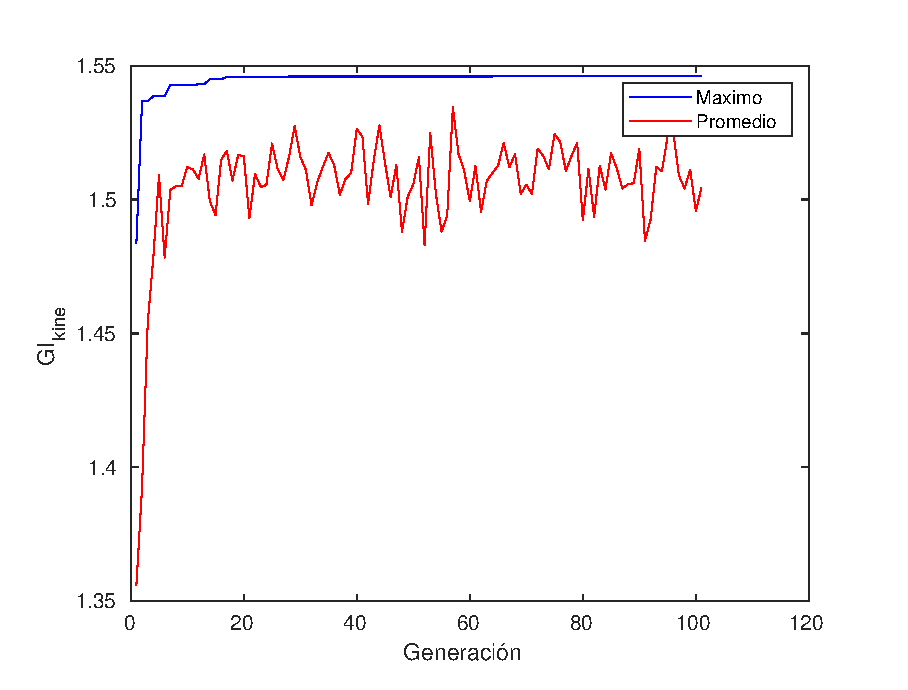
\includegraphics[height = 0.4\textheight,width=0.8\textwidth]{Cap4_DisenoBasico/Figura/Ga/IndiceenlasGeneraciones.eps}
    \caption{Indice Global de Desempeño Cinematico}
    \label{fig:Generaciones}
\end{figure}
\newpage
El algoritmo genetico de optimización se ejecuto 120 generaciones para una población de 25 cromosomas teniendo en cuenta las siguientes variables a optimizar y sus rangos de valores admisibles.\newline
$R_b$ = [500: 1000] mm \newline
$L_A$ = [50: 250] mm \newline
$L_D$ = [50: 250] mm \newline
$e$  = [-100: 100] mm \newline

Los resultados del algortimo genetico nos proporcionaron las siguientes medidas para un dimensionamiento optimo, obteniendo un indice global de desempeño cinematico de 1.5462 \newline
$R_b$ =  675.0946 mm \newline
$L_A$ = 50.0819 mm \newline
$L_D$ = 249.3099 mm \newline
$e$  = 0.0048 mm \newline

A continuación, se presenta la distribucion de los indices de desempeño de manera normalizada en el espacio de trabajo, apreciando los cambios de estos respecto a la solución inicial
\begin{figure}[ht!]
    \centering
    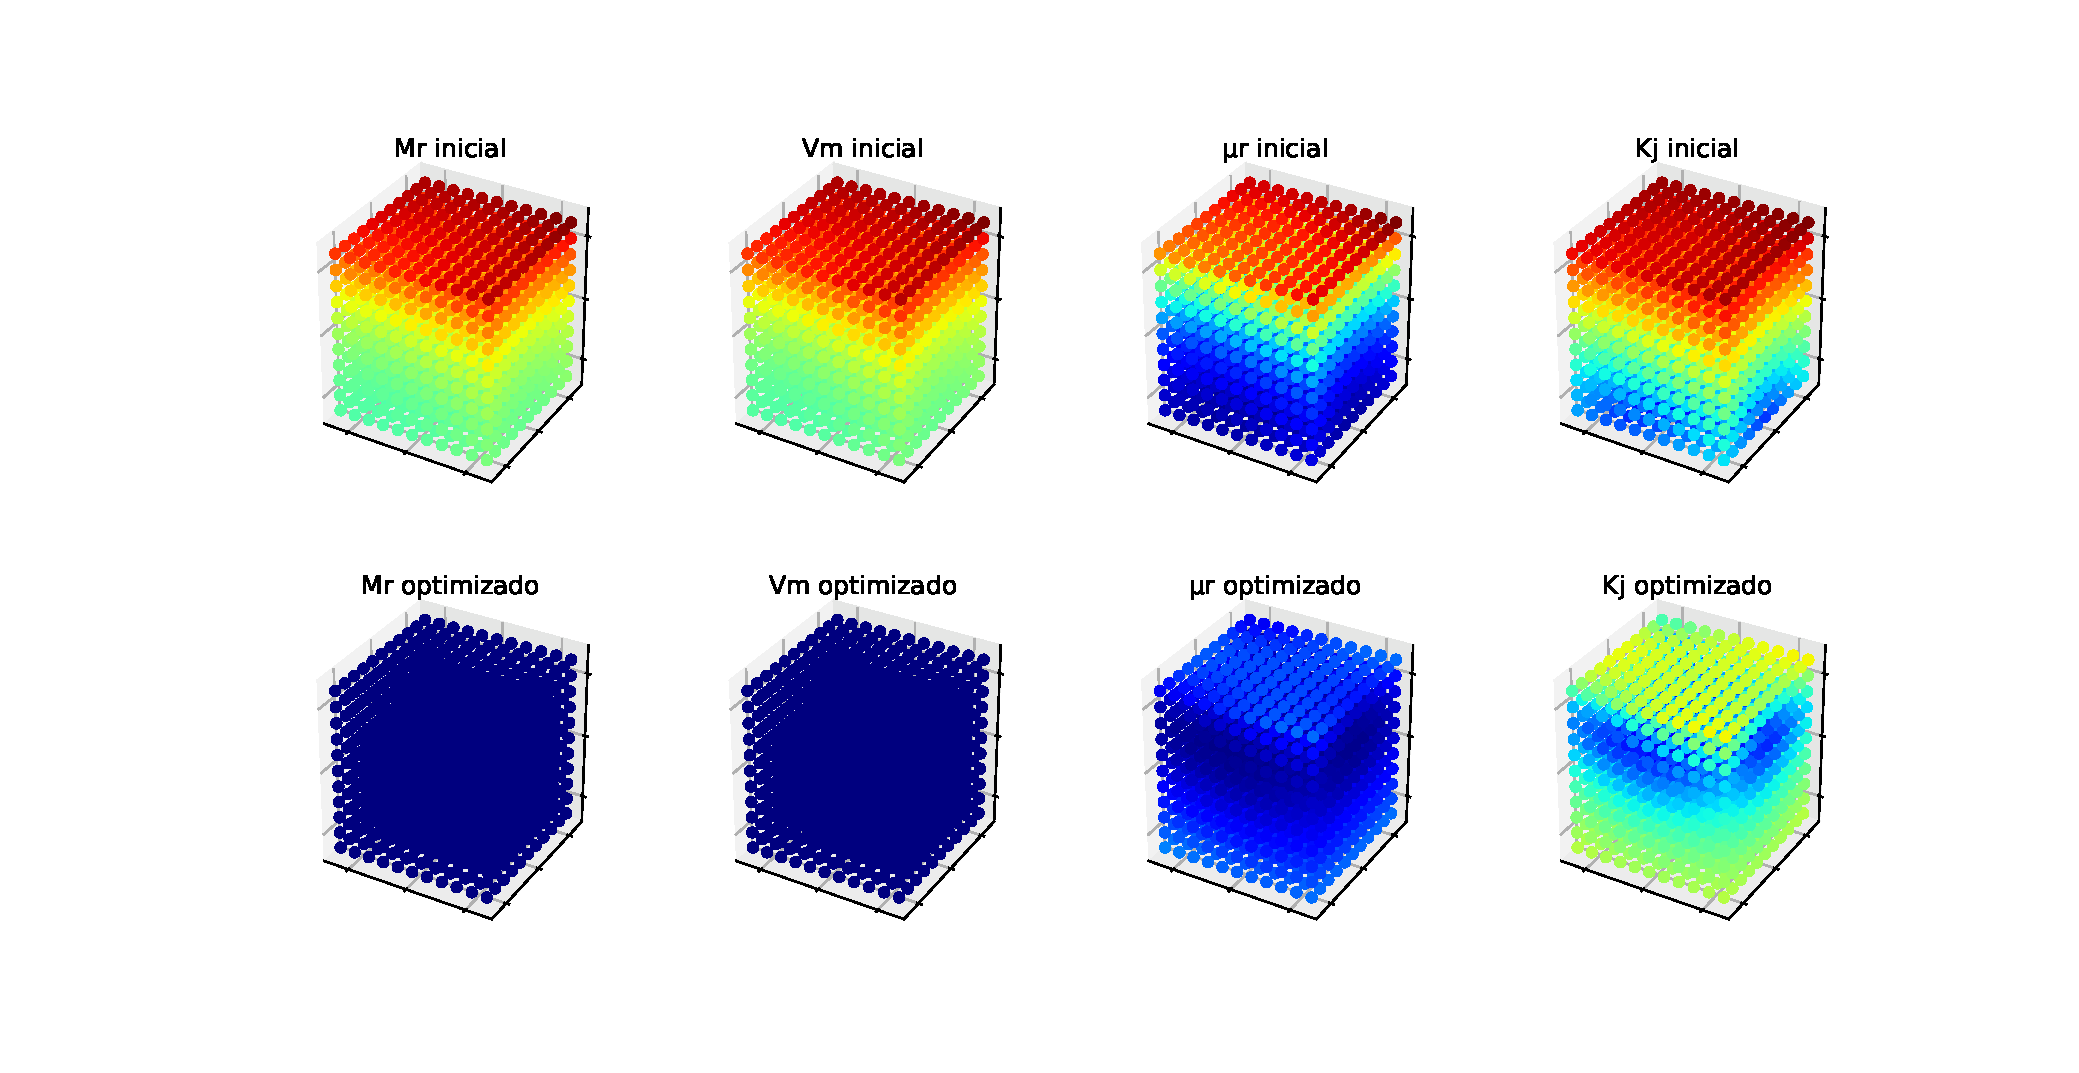
\includegraphics[height = 0.4\textheight,width=1\textwidth]{Cap4_DisenoBasico/Figura/Ga/Indices.eps}
     
\includegraphics[height = 0.04\textheight,width=0.7\textwidth]{Cap4_DisenoBasico/Figura/Ga/Colorbar.png}
    \caption{Indices de desempeño en el espacio de trabjo}
    \label{fig:optimization}
\end{figure}